\documentclass[]{article}
\usepackage{amssymb,amsmath}

\usepackage[style=verbose]{biblatex}
\addbibresource{biblio.bib}

\usepackage{pdflscape}

\usepackage{fontspec}
\defaultfontfeatures{Ligatures=TeX,Scale=MatchLowercase}
\setmainfont[]{cantarell}

\usepackage{graphicx}
\usepackage{wrapfig}
\usepackage{hyperref}
\urlstyle{same}  % don't use monospace font for urls
\usepackage[margin=4pt]{subcaption}

\usepackage[margin=2cm]{geometry}
\usepackage{longtable,booktabs}

\usepackage{pgfgantt}
\usepackage{rotating}

\usepackage{tocloft}

\renewcommand{\thesubsubsection}{}


\newcommand{\task}[2]{\vspace{0.5cm}\noindent\emph{Task T#1}: {\bf #2}\par}

\newcommand{\D}[3]{\emph{Deliverable D#1} (M#2): #3\\}

\newcommand{\TODO}[1]{{\color{red}\textbf{TODO: #1}}}

\newcommand{\severin}[1]{{\color{red}\textbf{Severin: #1}}}
\newcommand{\toseverin}[1]{{\color{red}\textbf{To Severin: #1}}}
\newcommand{\eu}[1]{{\color{teal}\textbf{Guidelines EU FET: #1}}}
\newcommand{\cellgrey}{\cellcolor[gray]{0.85}}


\title{WizMe - Part B}

\begin{document}
\maketitle

\subsection{Notes}

\paragraph ACAMH conference on Mental health and refugees:

Keywords:
\begin{itemize}
    \item Trauma
    \item Unaccompanied Asylum Seeking Children
\end{itemize}

Discussion with Helen Peden, Refugee Council, happy to contact
\begin{itemize}
    \item litteracy issues; example -> learn to read a map
    \item need to be primarily verbal
    \item work with 16/20 yo

\end{itemize}

\begin{itemize}
    \item 25M refugees, 50\% under 18
\end{itemize}

Good talk b Sarah Hunt (Uni Leicester)

\begin{itemize}
    \item Participatory Action Research ("From voice to agency", Rodriguez and
        Brown 2009)
    \item focus on post-migratory risk factors to mental health
    \item hceck photo of litterature review
    \item check participatory methodology (photos of slides)
    \item 3 themes emerging from her research: understanding trauma; need for
        responsive/individualised pathways; need for housing + basic needs
        provisions
    \item she mention lack of privacy in some provided housing as a permanent
        threat and a source of stress/trauma: \textbf{relation to privacy by
        design}
    \item point out the need to support not only the children but also the
        schools
    \item reference to World Awarness Children in Trauma Model (WACIT, Vostanis
        2012-2018)
    \item example of social integration issues: lack of knowledge of school
        rules (like raising ones' hands, perceived as bad behaviours/threatening
        behaviour); difficulty to meet with peers
    \item point raised about need for refugee children to 'fit in a new
        identity, matching local norms/expectation, at the cost of the previous,
        original identity -> source of suffering: importance of \emph{securing
        identity}, as done by some schools (example of school inviting parents
        of diverse background to come and cook home dishes at school, with
        different background every week)
\end{itemize}


Prof Ravi Kohli (child welfare):

\begin{itemize}
    \item Safety <-> belonging <-> success (cf photo)
    \item ...but not a straight line! Comes and go!
    \item underline the need by refugees to reciprocate
    \item make a strong point on individual identities instead of being just a label (cf
        photo)
    \item \textbf{importance of individual stories}
\end{itemize}

Powerful presentation by Bobby Lloyds; she stayed 2 days/week for 4 years in
Calais camp; visual artist + art therapist; large archive of field experience on
Facebook account (ArtRefuge UK)

She points out the importance of mobile phones -> communication, story telling,
etc


\subsection*{Title of the proposal}\label{title-of-the-proposal}

\textbf{Social robots to support human-human interactions}

\subsection*{Acronym}\label{acronym}

WizMe

\subsection*{Abstract}\label{abstract}

WizMe is a future-looking project that aims at investigating how social
robots can shape and support stronger \emph{human-human} relationships:
in a time where robots are on the verge of becoming pervasive in our
environment, can we use them as powerful tool to develop rich, positive human
interactions as well?


Such robots require unique, beyond state-of-the-art, capabilities to
\emph{(1)} understand the social interactions (\emph{social situation
awareness}), \emph{(2)} decide the best course of action for short-term
and longer-term social influence, and \emph{(3)} perform the appropriate
social acts and exert adequate, ethical social influence.

In the WizMe project, we propose to scaffold this radically novel line
of research with an original application of high societal impact: we
will create a small set of novel personal companion robots designed to
facilitate human-human interactions. These robots will be deployed in
selected school to support the social and cultural integration of
vulnerable children, with a particular focus on migrant children who
might lack the otherwise needed support for a successful integration
(different cultures and social norms; absence of local, culturally
integrated, relatives; language barriers; etc.).

This project is ambitious, and brings together five leading groups in
social human-robot interaction, interaction design and human
socio-developmental psychology, with unique expertise and contributions:
The Bristol Robotics Lab, the largest UK robotic lab, has a long history
of running and leading complex projects involving hardware, software and
AI, with a strong track record in human-robot interaction and assistive
robotics; the University of Ghent will provide world-leading expertise
on robot design for interaction with children; the EPFL's CHILI lab has
a unique expertise in blending technology (and social robotics in
particular) in teaching environments, with a focus on rich social
interaction; the IST is recognised as a leading group in expressive
social agents and also has a very strong track record in child-robot
interactions; finally {[}socio-psychology partner{]}.

Critically, the complex interaction design that lies at the core of the
project will be informed and co-led by the Refugee Support department of
RedCross UK, one of the largest NGO world-wide.

\pagebreak

%%%%%%%%%%%%%%%%%%%%%%%%%%%%%%%%%%%%%%%%%%%%%%%%%%%%%%%%%%%%%%%%%%%%%%%%%%%%%%%%%%%%%%%%
%%%%%%%%%%%%%%%%%%%%%%%%%%%%%%%%%%%%%%%%%%%%%%%%%%%%%%%%%%%%%%%%%%%%%%%%%%%%%%%%%%%%%%%%
%%%%%%%%%%%%%%%%%%%%%%%%%%%%%%%%%%%%%%%%%%%%%%%%%%%%%%%%%%%%%%%%%%%%%%%%%%%%%%%%%%%%%%%%
\section{Excellence}\label{part1}
\eu{(max 5 pages)}



\subsection{Long-term vision and targeted breakthrough towards that vision}

\begin{figure}[!htbp]
    \centering
    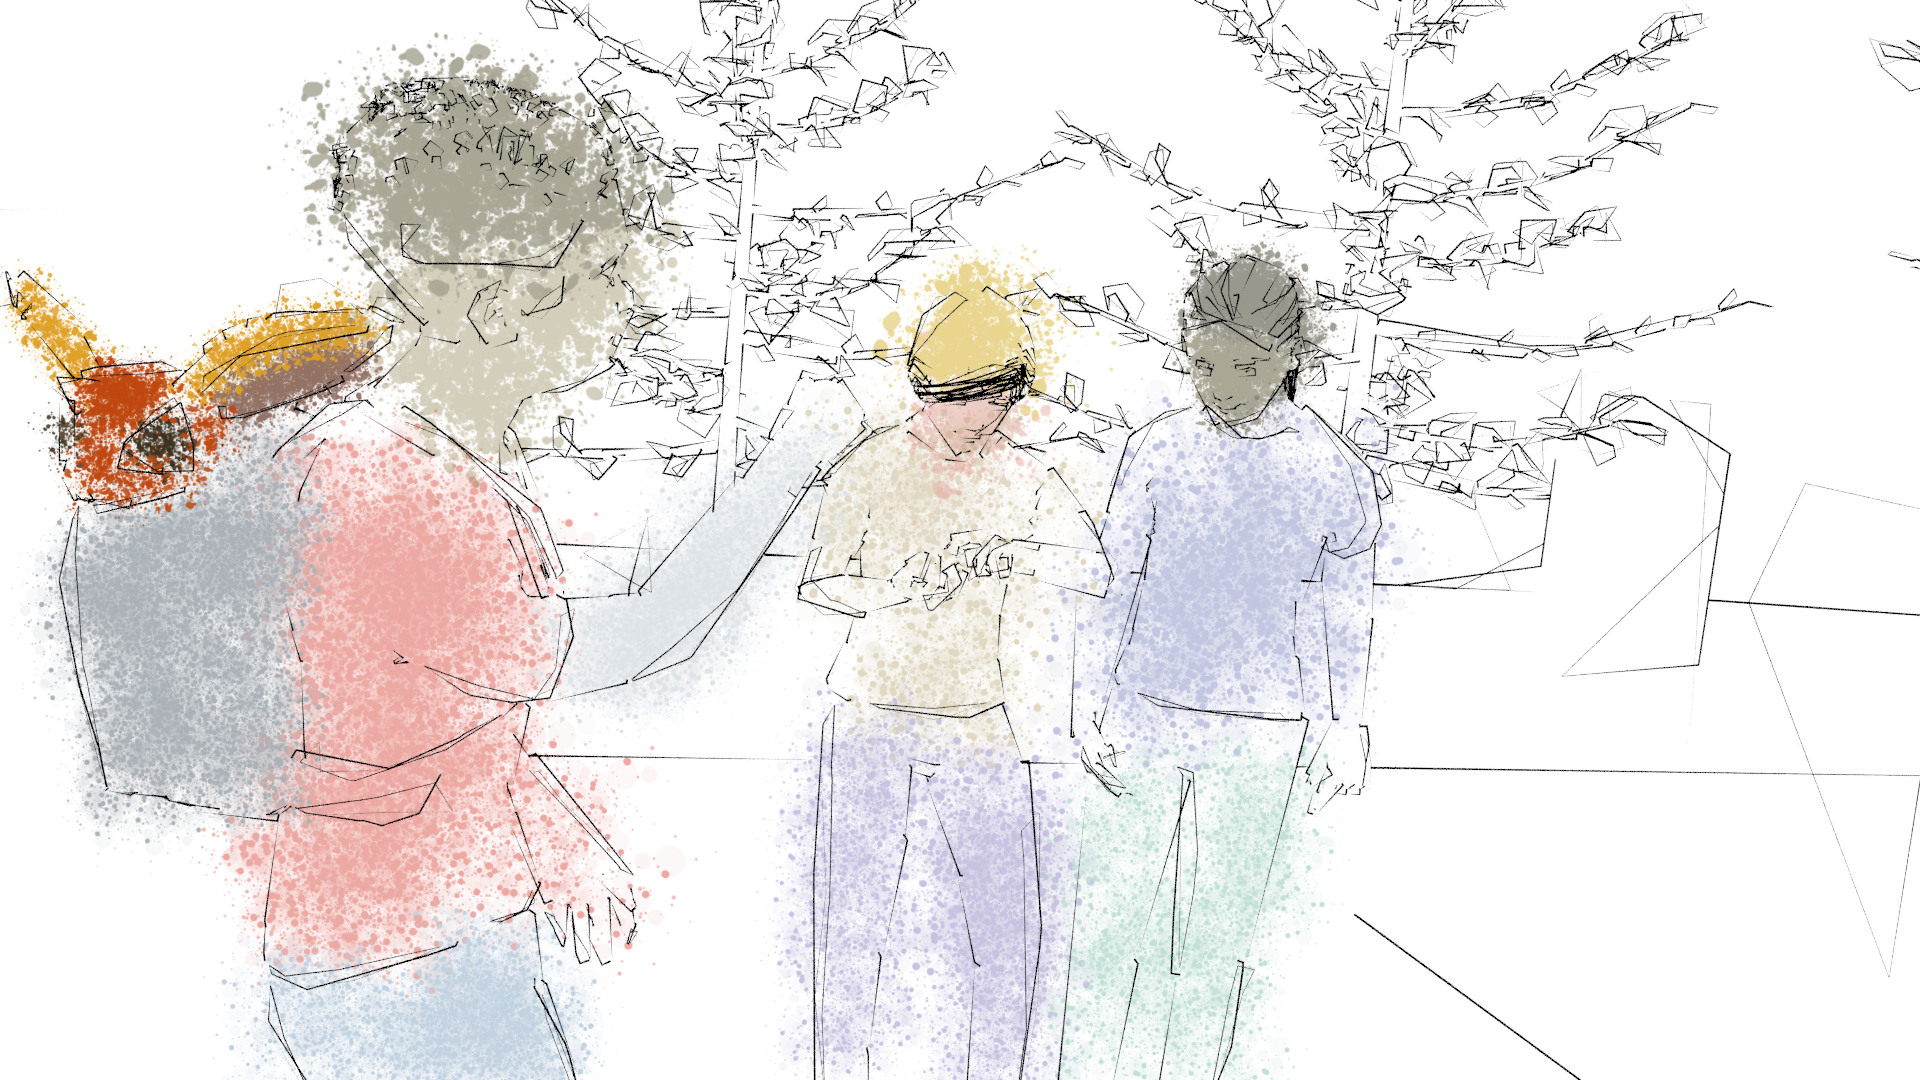
\includegraphics[width=0.9\linewidth]{figs/render5-colors.png}
\end{figure}

WizMe is a project that aims at helping to build strong human
relationships with the help of technology.

The core idea of the project is to build small companion robots whose
aim is to facilitate human-human interactions. We want to develop these
robots with a particular application in mind: supporting the social and
cultural integration of vulnerable children in a foreign country, and in
particular, migrant children who might lack the otherwise needed support
(shared culture; already well integrated relatives) for a successful
integration.

\subsubsection{Key scientific research questions}

\begin{enumerate}
\item research the role of social influence to scaffold positive human-human
    interactions (including its ethical ramifications) in the context of migrant
    integration;
\item explore how a small robot companion can be endowed with social
    competencies to positively influence human interactions; design and
    implement the corresponding artificial social behaviours;
\item design and build a small rugged and autonomous companion robot that
    realise this goal for child-child interactions; test the technology in
    school with actual migrant children.
\end{enumerate}

\subsubsection{Vision of a novel form of interaction ``human-(robot)-human''}

\paragraph{The case of the social integration of migrant children}

A robot is left with the child when he or she starts their journey in
their new host country, and becomes a companion for the child during the
first months of the integration. Using several mechanisms that are
discussed in this proposal, the robot helps the child to gain
self-confidence, and ultimately engage in successful social interactions
with other children.

Critically, the robot is designed to support the social and cultural
integration of the child \emph{amongst her/his peers}. While the child
might build affective/emotional bonds with the robot over the course of
the support period, the robot behaviour is designed to ensure that these
bonds do not substitute themselves to the interactions with other
children.

The project combines a range of scientific and engineering endeavours to
realise within a 5-years timeframe an ambitious and bold vision for
social robotics in our society. Specifically, the project draws from the
fields of social robotics; human-robot interaction; human-machine
interaction design; and mechatronics.

While the breadth of the proposed project is significant (from
mechatronic design to long-term field testing with vulnerable
populations), the project structure minimizes the cross-dependencies
within the project, avoiding critical failure points that would put the
whole project at risk, and a careful risk assessment is conducted that
includes meaningful mitigation strategies.


\subsection{Novelty, non-incrementality, plausibility and foundational character}

\subsubsection{Companion robots}

One example of a small, rugged robot designed for intensive use in school
environments is Cellulo~\footcite{ozgur2017cellulo}.

\begin{figure}[!htbp]
    \begin{minipage}[b]{.3\linewidth}
        \centering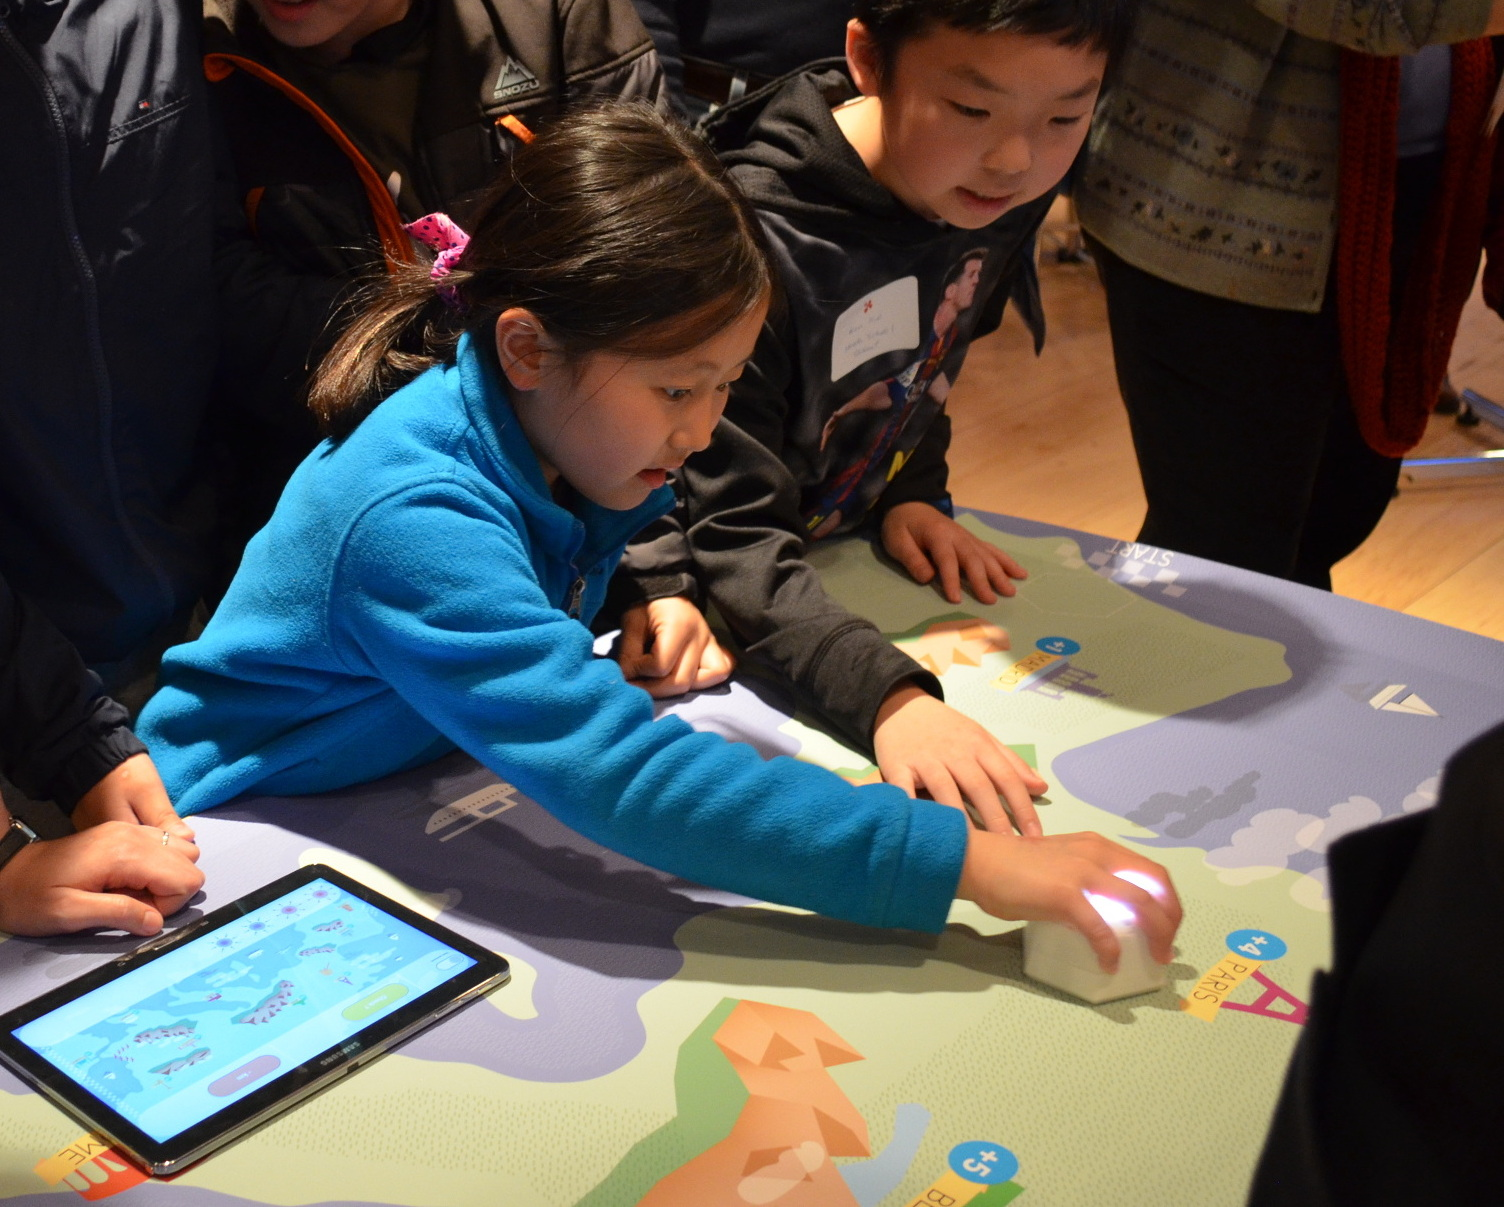
\includegraphics[height=4cm]{figs/cellulo.jpg}
        \subcaption{EPFL's Cellulo robot}\label{fig:cellulo}
    \end{minipage}%
    \hspace{0.5cm}
    \begin{minipage}[b]{.3\linewidth}
        \centering
        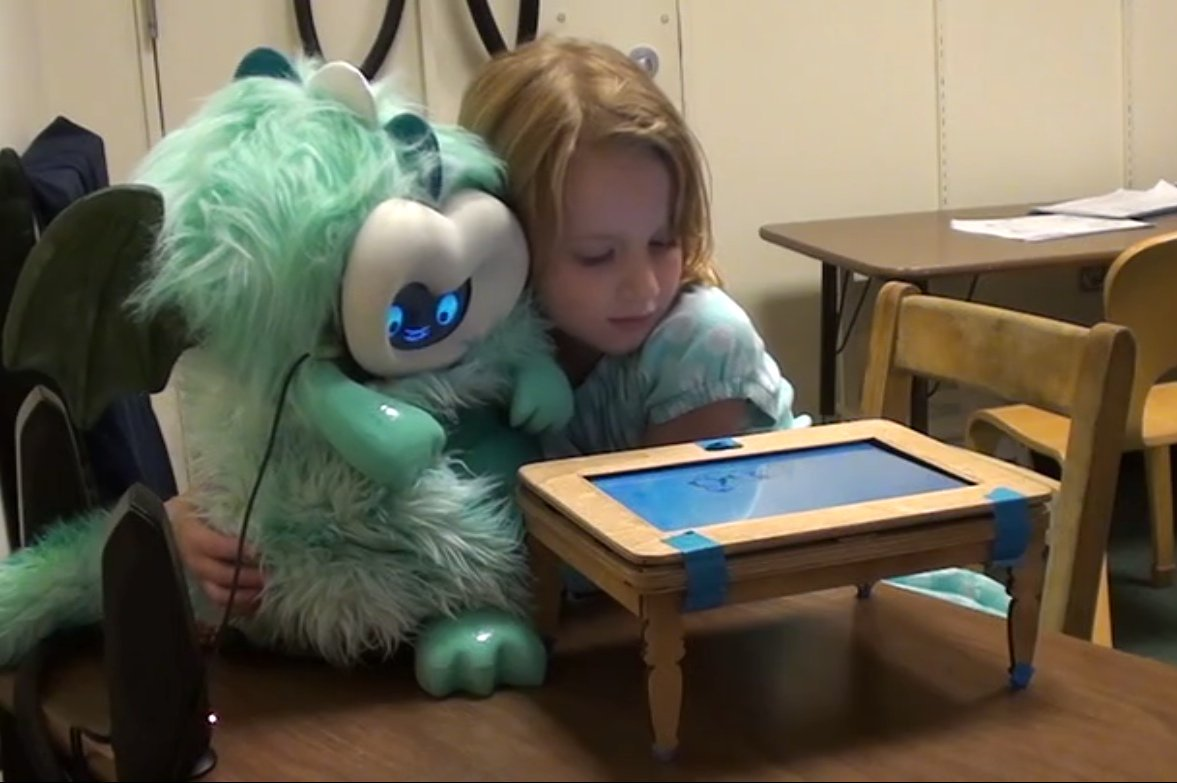
\includegraphics[height=4cm]{figs/tega.jpg}
        \subcaption{MediaLab's Tega robot}\label{fig:tega}
    \end{minipage}
    \hspace{0.5cm}
    \begin{minipage}[b]{.3\linewidth}
        \centering
        \includegraphics[height=4cm]{figs/ono.png}
        \subcaption{OPSORO's Ono robot}\label{fig:ono}
    \end{minipage}
    \caption{Existing research-level companion robots}\label{fig:research-robots}
\end{figure}

\begin{figure}[!htbp]
    \begin{minipage}[b]{.3\linewidth}
        \centering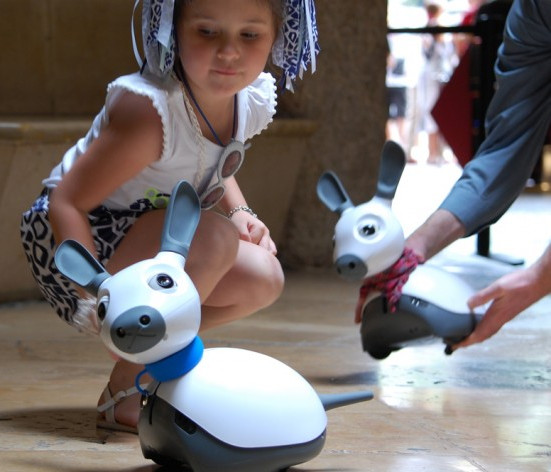
\includegraphics[height=4cm]{figs/miro.jpg}
        \subcaption{Consequential's Miro robot}\label{fig:miro}
    \end{minipage}%
    \hspace{0.1cm}
    \begin{minipage}[b]{.3\linewidth}
        \centering
        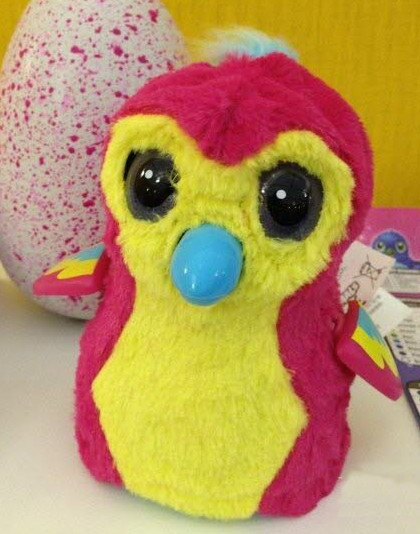
\includegraphics[height=4cm]{figs/hatchnimals.jpg}
        \subcaption{SpinMaster's Hatchimals}\label{fig:hatchimals}
    \end{minipage}%
    \hspace{0.1cm}
    \begin{minipage}[b]{.3\linewidth}
        \centering
        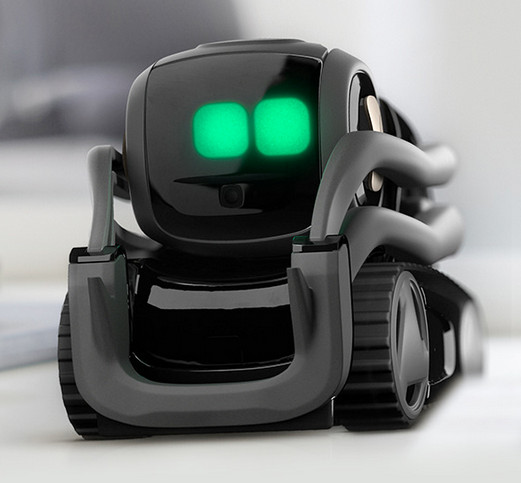
\includegraphics[height=4cm]{figs/anki-vector.jpg}
        \subcaption{Anki's Vector}\label{fig:vector}
    \end{minipage}
    \caption{Existing commercial companion robots}\label{fig:commercial-robots}
\end{figure}

\subsubsection{Social influence}

\begin{figure}[!htbp]
\centering
    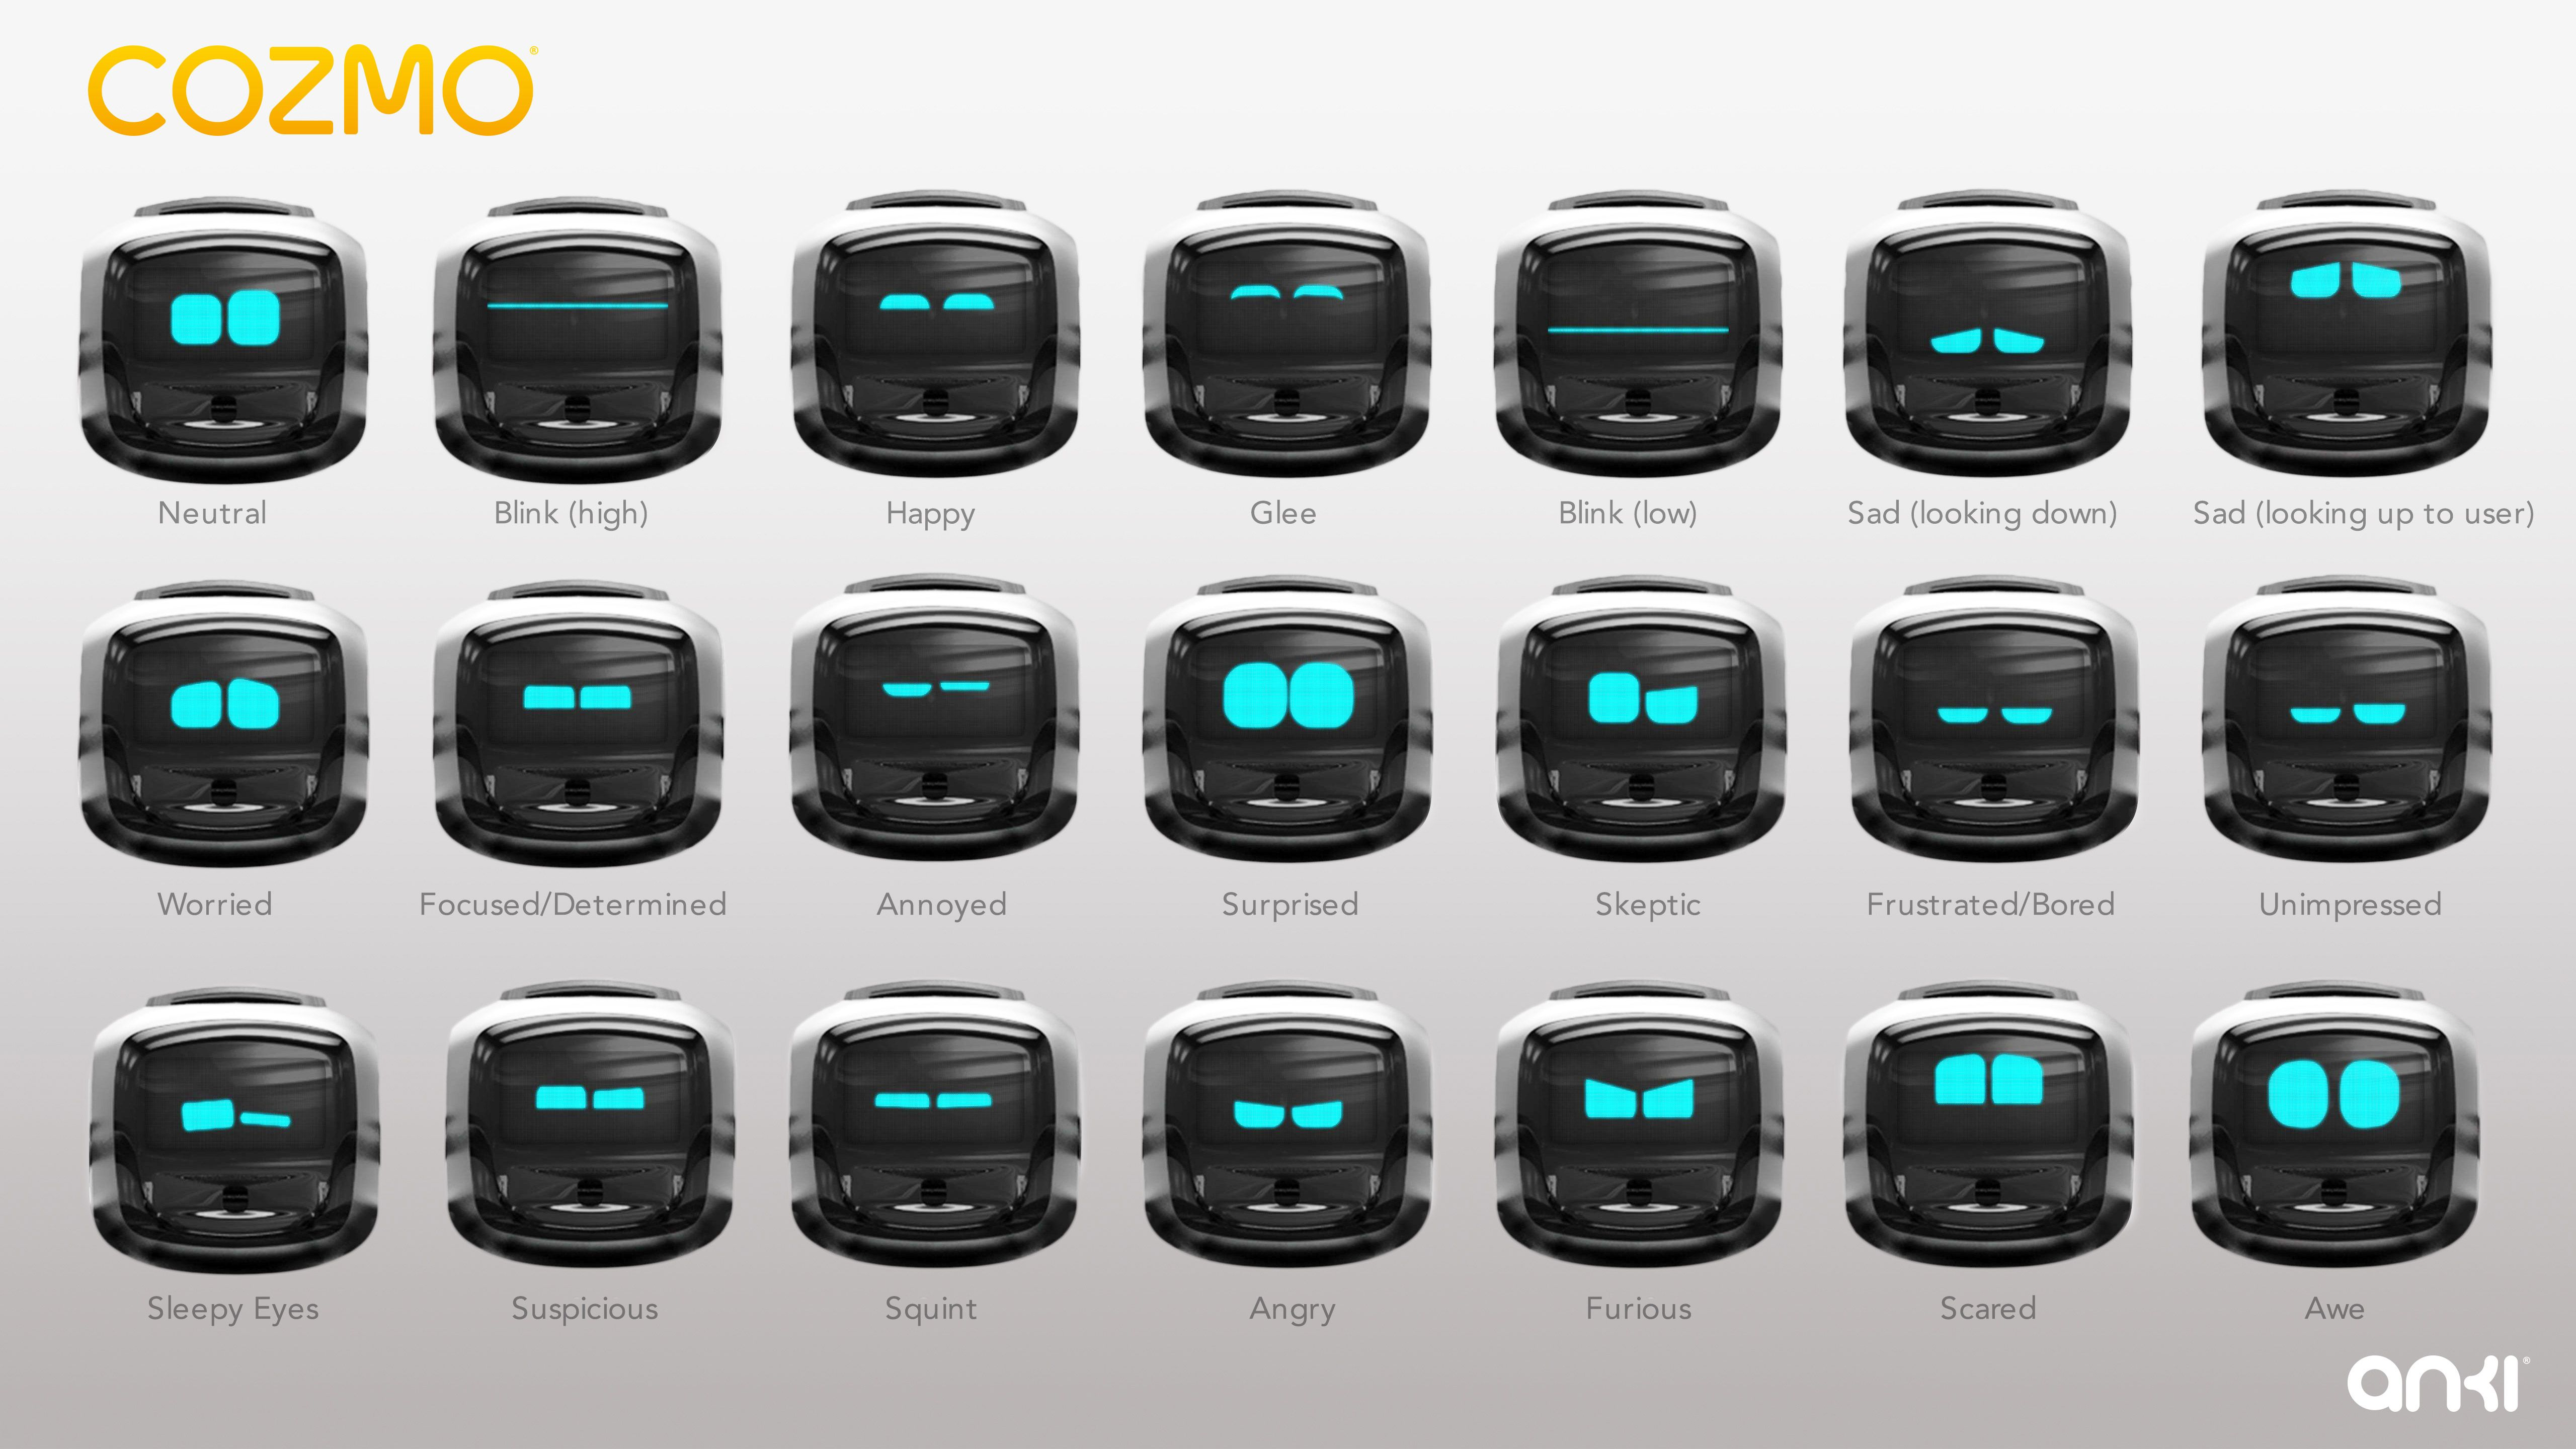
\includegraphics[width=0.7\textwidth]{figs/cozmo-expression-sheet.jpg}
\caption{Cozmo facial expressions}
\end{figure}


\subsection{Research methodology}\label{research-methodology}


\subsubsection{Deployments in schools}

\subsection{Interdisciplinarity}
%%%%%%%%%%%%%%%%%%%%%%%%%%%%%%%%%%%%%%%%%%%%%%%%%%%%%%%%%%%%%%%%%%%%%%%%%%%%%%%%%%%%%%%%
%%%%%%%%%%%%%%%%%%%%%%%%%%%%%%%%%%%%%%%%%%%%%%%%%%%%%%%%%%%%%%%%%%%%%%%%%%%%%%%%%%%%%%%%
%%%%%%%%%%%%%%%%%%%%%%%%%%%%%%%%%%%%%%%%%%%%%%%%%%%%%%%%%%%%%%%%%%%%%%%%%%%%%%%%%%%%%%%%

\newpage
\section{Impact}\label{impact}

\subsection{Impact on society and technology: building an inclusive society}

\subsection{Impact on future leadership}

\subsection{Measures for achieving impact}

\subsubsection{Dissemination and exploitation of results}

\subsubsection{Communication activities}


%%%%%%%%%%%%%%%%%%%%%%%%%%%%%%%%%%%%%%%%%%%%%%%%%%%%%%%%%%%%%%%%%%%%%%%%%%%%%%%%%%%%%%%%
%%%%%%%%%%%%%%%%%%%%%%%%%%%%%%%%%%%%%%%%%%%%%%%%%%%%%%%%%%%%%%%%%%%%%%%%%%%%%%%%%%%%%%%%
%%%%%%%%%%%%%%%%%%%%%%%%%%%%%%%%%%%%%%%%%%%%%%%%%%%%%%%%%%%%%%%%%%%%%%%%%%%%%%%%%%%%%%%%
\newpage
\section{Implementation}\label{part3}

%%%%%%%%%%%%%%%%%%%%%%%%%%%%%%%%%%%%%%%%%%%%%%%%%%%%%%%%%%%%%%%%%%%%%%%%%%%%%%%%%%%%%%%
%% Names of the Work packages

\newcommand{\wpOne}{Project management}
\newcommand{\wpOneShort}{\wpOne{}}

\newcommand{\wpTwo}{Technology to socially influence human-human interactions}
\newcommand{\wpTwoShort}{Social influence}


\newcommand{\wpThree}{Interaction design for robot-supported human-human interactions}
\newcommand{\wpThreeShort}{Interaction design}

\newcommand{\wpFour}{Design and building of a companion robot for social interaction in the field}
\newcommand{\wpFourShort}{Companion robot creation}

\newcommand{\wpFive}{AI for social cognition}
\newcommand{\wpFiveShort}{AI for social cognition}

\newcommand{\wpSix}{Dissemination and exploitation}
\newcommand{\wpSixShort}{Dissemination}


%%%%%%%%%%%%%%%%%%%%%%%%%%%%%%%%%%%%%%%%%%%%%%%%%%%%%%%%%%%%%%%%%%%%%%%%%%%%%%%%%%%%%%%


\subsection{Workplan and intermediate targets}

\subsubsection{Project structure}

\begin{table}[!htbp]
    \begin{tabular}{@{}p{1cm}p{6cm}p{2cm}p{2cm}p{1.5cm}p{1.5cm}p{1.5cm}@{}}
\toprule
\textbf{WP} & \textbf{Work package title} & \textbf{Lead participant No} & \textbf{Lead participant short name} & \textbf{Person-Months} & \textbf{Start month} & \textbf{End month} \\ \midrule
1                        & \wpOne                      &                              &                                      &                        &                      &                    \\
2                        & \wpTwo                      &                              &                                      &                        &                      &                    \\
3                        & \wpThree                    &                              &                                      &                        &                      &                    \\
4                        & \wpFour                     &                              &                                      &                        &                      &                    \\
5                        & \wpFive                     &                              &                                      &                        &                      &                    \\
6                        & \wpSix                      &                              &                                      &                        &                      &                    \\
                         &                             &                              &                                      & \textbf{Total months}  &                      &                    \\ \bottomrule
\end{tabular}
\end{table}


\subsubsection{Work package 1: \wpOne}

\begin{table}[!htbp]
\centering
\begin{tabular}{|l|p{1.5cm}|p{1.5cm}|p{1.5cm}|p{1.5cm}|p{1.5cm}|p{1.5cm}|p{1.5cm}|}
\hline
Work package number            & 1 & \multicolumn{3}{l|}{Lead beneficiary} & \multicolumn{3}{l|}{\bf BRL} \\ \hline
Work package title             & \multicolumn{7}{l|}{\wpOne}                                             \\ \hline
Participant number             &     &         &         &                  &       &       &      \\ \hline
Short name of participant      &     &         &         &                  &       &       &      \\ \hline
Person/months per participant: &     &         &         &                  &       &       &      \\ \hline
Start month                    & \multicolumn{3}{l|}{}  & End month        & \multicolumn{3}{l|}{} \\ \hline
\end{tabular}
\end{table}


\textbf{Objectives:}

\textbf{Description of work:}

\ldots{}description\ldots{}

\task{1.1}{}

\vspace{0.5cm}\textbf{Deliverables:}

\begin{itemize}

\item   \emph{Deliverable D1.1} (Month 2): website and logo
\end{itemize}

\subsubsection{Work package 2: \wpTwo}

\begin{table}[!htbp]
\centering
\begin{tabular}{|l|p{1.5cm}|p{1.5cm}|p{1.5cm}|p{1.5cm}|p{1.5cm}|p{1.5cm}|p{1.5cm}|}
\hline
Work package number            & 2 & \multicolumn{3}{l|}{Lead beneficiary} & \multicolumn{3}{l|}{} \\ \hline
Work package title             & \multicolumn{7}{l|}{\wpTwo}                                       \\ \hline
Participant number             &     &         &         &                  &       &       &      \\ \hline
Short name of participant      &     &         &         &                  &       &       &      \\ \hline
Person/months per participant: &     &         &         &                  &       &       &      \\ \hline
Start month                    & \multicolumn{3}{l|}{}  & End month        & \multicolumn{3}{l|}{} \\ \hline
\end{tabular}
\end{table}

\textbf{Objectives:}
\textbf{Description of work:}

\ldots{}description\ldots{}

\task{2.1}{Identification of the dimensions of social influence for human interpersonal interactions}

\task{2.2}{Ethics of social influence}
Blah blah

\task{2.3}{Study 1 -- Socially influencing companion robot}
First study, using Anki's Vector robot.

\vspace{0.5cm}\textbf{Deliverables:}

\begin{itemize}
    \item \D{2.1}{12}{great report}
\end{itemize}

\subsubsection{Work package 3: \wpThree}

\begin{table}[!htbp]
\centering
\begin{tabular}{|l|p{1.5cm}|p{1.5cm}|p{1.5cm}|p{1.5cm}|p{1.5cm}|p{1.5cm}|p{1.5cm}|}
\hline
Work package number            & 3 & \multicolumn{3}{l|}{Lead beneficiary} & \multicolumn{3}{l|}{} \\ \hline
Work package title             & \multicolumn{7}{l|}{\wpThree}                                     \\ \hline
Participant number             &     &         &         &                  &       &       &      \\ \hline
Short name of participant      &     &         &         &                  &       &       &      \\ \hline
Person/months per participant: &     &         &         &                  &       &       &      \\ \hline
Start month                    & \multicolumn{3}{l|}{}  & End month        & \multicolumn{3}{l|}{} \\ \hline
\end{tabular}
\end{table}

\textbf{Objectives:}

\begin{itemize}
    \item refine interaction modalities (in
    particular, the non-verbal speech), details cross-modal interactions,
    define interaction patterns with the child
\end{itemize}

\ldots{}description\ldots{}

\task{3.1}{Analysis of needs}
\task{3.2}{Cross-cultural interactions}

\vspace{0.5cm}\textbf{Deliverables:}

\begin{itemize}
    \item \D{3.1}{12}{great report}
\end{itemize}

\subsubsection{Work package 4: \wpFour}

\begin{table}[!htbp]
\centering
\begin{tabular}{|l|p{1.5cm}|p{1.5cm}|p{1.5cm}|p{1.5cm}|p{1.5cm}|p{1.5cm}|p{1.5cm}|}
\hline
Work package number            & 4 & \multicolumn{3}{l|}{Lead beneficiary} & \multicolumn{3}{l|}{} \\ \hline
Work package title             & \multicolumn{7}{l|}{\wpFour}                                      \\ \hline
Participant number             &     &         &         &                  &       &       &      \\ \hline
Short name of participant      &     &         &         &                  &       &       &      \\ \hline
Person/months per participant: &     &         &         &                  &       &       &      \\ \hline
Start month                    & \multicolumn{3}{l|}{}  & End month        & \multicolumn{3}{l|}{} \\ \hline
\end{tabular}
\end{table}


\begin{itemize}
    \item long term interaction
    \item one full day of autonomy
    \item rugged \footcite{ozgur2017cellulo, hostettler2016realtime}
    \item child friendly: mechanical constraints~\footcite{ozgur2016permanent} + design
\end{itemize}


\textbf{Description of work:}

Develop a novel platform, including:

\begin{itemize}
    \item chassis
    \item power autonomy for one day
    \item on-board compute suitable for deep learning (NVidia Xavier?)
    \item vision (embedded RGB-D camera)
    \item audio processing
\end{itemize}

\ldots{}

\task{4.1}{Physical design of the robot companion}
\task{4.2}{Interaction design}
\task{4.3}{Mechatronics \& Sensing}
\task{4.4}{On-board data processing}
\task{4.5}{System integration}

\begin{itemize}
    \item \D{4.1}{12}{great report}
\end{itemize}

\subsubsection{Work package 5: \wpFive}

\begin{table}[!htbp]
\centering
\begin{tabular}{|l|p{1.5cm}|p{1.5cm}|p{1.5cm}|p{1.5cm}|p{1.5cm}|p{1.5cm}|p{1.5cm}|}
\hline
Work package number            & 5 & \multicolumn{3}{l|}{Lead beneficiary} & \multicolumn{3}{l|}{} \\ \hline
Work package title             & \multicolumn{7}{l|}{\wpFive}                                      \\ \hline
Participant number             &     &         &         &                  &       &       &      \\ \hline
Short name of participant      &     &         &         &                  &       &       &      \\ \hline
Person/months per participant: &     &         &         &                  &       &       &      \\ \hline
Start month                    & \multicolumn{3}{l|}{}  & End month        & \multicolumn{3}{l|}{} \\ \hline
\end{tabular}
\end{table}


\textbf{Objectives:}

\textbf{Description of work:}

\ldots{}description\ldots{}

\task{5.1}{Multi-modal communication}
\task{5.2}{Social awareness}
\task{5.3}{Machine learning of social behaviours}
\task{5.4}{Social controller}

\vspace{0.5cm}\textbf{Deliverables:}

\begin{itemize}
    \item \D{5.1}{12}{great report}
\end{itemize}

\subsubsection{Work package 6: \wpSix}

\begin{table}[!htbp]
\centering
\begin{tabular}{|l|p{1.5cm}|p{1.5cm}|p{1.5cm}|p{1.5cm}|p{1.5cm}|p{1.5cm}|p{1.5cm}|}
\hline
Work package number            & 6 & \multicolumn{3}{l|}{Lead beneficiary} & \multicolumn{3}{l|}{} \\ \hline
Work package title             & \multicolumn{7}{l|}{\wpSix}                                       \\ \hline
Participant number             &     &         &         &                  &       &       &      \\ \hline
Short name of participant      &     &         &         &                  &       &       &      \\ \hline
Person/months per participant: &     &         &         &                  &       &       &      \\ \hline
Start month                    & \multicolumn{3}{l|}{}  & End month        & \multicolumn{3}{l|}{} \\ \hline
\end{tabular}
\end{table}


\textbf{Objectives:}

\textbf{Description of work:}

\ldots{}description\ldots{}

\task{6.1}{Academic dissemination}
\task{6.2}{General public dissemination}
\task{6.3}{Commercial exploitation}

\vspace{0.5cm}\textbf{Deliverables:}

\begin{itemize}
    \item \D{6.1}{12}{website and logo}
\end{itemize}

\subsubsection{Deliverables overview}\label{deliverables-overview}

\begin{table}[!htbp]
\caption{List of deliverables}
\begin{tabular}{@{}lllllll@{}}
\toprule
\textbf{Deliverable} & \textbf{Deliverable name} & \textbf{Work package No} & \textbf{Lead participant short name} & \textbf{Type} & \textbf{Dissemination level} & \textbf{Delivery date} \\ \midrule
D1.1                 &                           &                          &                                      &               &                              &                        \\
D1.2                 &                           &                          &                                      &               &                              &                        \\
D2.1                 &                           &                          &                                      &               &                              &                        \\
...                  &                           &                          &                                      &               &                              &                        \\ \bottomrule
\end{tabular}
\end{table}

Type:

\begin{itemize}

\item   R: Document, report (excluding the periodic and final reports)
\item   DEM: Demonstrator, pilot, prototype, plan designs
\item   DEC: Websites, patents filing, press \& media actions, videos, etc.
\item   OTHER: Software, technical diagram, etc.
\end{itemize}

Dissemination level:

\begin{itemize}

\item   PU = Public, fully open, e.g.~web
\item   CO = Confidential, restricted under conditions set out in Model Grant
  Agreement
\item   CI = Classified, information as referred to in Commission Decision
  2001/844/EC.
\end{itemize}

\subsubsection{Gantt chart}\label{gantt-chart}

\begin{landscape}
%%%%%%%%%%%%%%%%%
%%
%% Task dependencies
%%
%% Task...        depends on Task...
%% T1.3           T1.1
%% T1.3           T1.2
%% T1.2           T2.2 (user interface)
%% T3.3           T2.3
%%

\definecolor{barcolor}{RGB}{153,204,254}
\definecolor{linkred}{RGB}{165,0,33}
%\renewcommand\sfdefault{phv}
%\renewcommand\mddefault{mc}
%\renewcommand\bfdefault{bc}
\setganttlinklabel{s-s}{START-TO-START}
\setganttlinklabel{f-s}{}
\setganttlinklabel{f-f}{FINISH-TO-FINISH}

%\begin{sidewaysfigure}[!ht]
\begin{figure}[!ht]

%\sffamily
\begin{ganttchart}[
        canvas/.append style={fill=none, draw=black!5, line width=.75pt},
        hgrid style/.style={draw=black!5, line width=.75pt},
        vgrid={*1{draw=black!5, line width=.75pt}},
        %vgrid={*1{black}, *{11}{black!5}}, % doesnt work for some reason
        x unit=.35cm,
        y unit chart=.65cm,
        time slot format=isodate-yearmonth,
        time slot unit=month, % pgfgantt >= 5.0
        %compress calendar, % pgfgantt < 5.0 => overleaf
        title/.style={draw=none, fill=none},
        title label font=\bfseries\footnotesize,
        %title label node/.append style={below=7pt},
        include title in canvas=false,
        bar label font=\mdseries\small\color{black!70},
        %bar label node/.append style={left=2cm},
        bar/.append style={draw=none, fill=barcolor!50},
        bar progress label font=\mdseries\footnotesize\color{black!70},
        group/.append style={fill=barcolor},
        group incomplete/.append style={fill=black},
        group left shift=0,
        group right shift=0,
        group height=.5,
        group peaks tip position=0,
        group label node/.append style={left=.6cm},
        group progress label font=\bfseries\small,
        link/.style={-latex, line width=1.5pt, linkred},
        link label font=\scriptsize\bfseries,
        link label node/.append style={below left=-2pt and 0pt,
        milestone/.append style={circle},
        milestone inline label node/.append style={left=5mm}}
    ]{2021-01}{2025-12}
    
        %\gantttitle[
        %    title label node/.append style={below left=7pt and -3pt}
        %]{Month:\quad1}{1}
        \gantttitlecalendar{year, month} \\
        %\gantttitlelist{0,5,...,60}{1} \\
        %% WP1
        \ganttgroup[]{WP1 \wpOneShort}{2021-01}{2023-12} \\
            \ganttbar[name=WP11]{\textbf{1.1} Conceptual framing \& ethics}{2021-01}{2023-12} \\
            \ganttbar[name=WP12prep,inline,bar/.append style={fill=gray!20}]{preparation}{2021-07}{2021-12}
            \ganttbar[name=WP12exp,inline]{WeTheCurious experiment}{2022-01}{2022-12}
            \ganttbar[name=WP12]{\textbf{1.2} Principles of r-HHI}{2023-01}{2023-06} \\

        %\ganttlink[link type=f-s]{WBS1A}{WBS1B}

        %% WP2
        \definecolor{barcolor}{RGB}{153,2,254}
        \ganttgroup[]{WP2 \wpTwoShort}{2021-01}{2024-12} \\
            \ganttbar[name=WP21]{\textbf{2.1} Situation assessment}{2021-01}{2022-06} \\
            \ganttbar[name=WP22]{\textbf{2.2} Social dynamics}{2022-01}{2023-12} \\
            \ganttbar[name=WP23]{\textbf{2.3} Group dynamics}{2024-01}{2024-12} \\
            \ganttbar[name=WP24]{\textbf{2.4} Social situation assessment}{2022-07}{2024-12} \\

        %\ganttlink[link type=f-s]{WP21}{WP24}
        %\ganttlink[link type=f-s]{WP22}{WP23}

        %% WP3
        \definecolor{barcolor}{RGB}{50,220,134}
        \ganttgroup[]{WP3 \wpThreeShort}{2021-01}{2025-12} \\
            \ganttbar[name=WP31]{\textbf{3.1} Social teleology}{2023-01}{2024-12} \\
            \ganttbar[name=WP32]{\textbf{3.2} Human-in-the-loop policy learning}{2021-07}{2025-06} \\
            \ganttbar[name=WP33]{\textbf{3.3} Integrated cognitive architecture}{2021-01}{2025-06} \\

        %\ganttlink[link type=f-s]{WP12}{WP32}

        %% WP4
        \definecolor{barcolor}{RGB}{244,50,20}
        \ganttgroup[]{WP4 \wpFourShort}{2022-01}{2025-12} \\
            \ganttbar[name=WP41]{\textbf{4.1} Behaviours baselining}{2022-01}{2022-12} \\
            \ganttbar[name=WP42]{\textbf{4.2} Generative behaviours}{2023-01}{2023-12} \\
            \ganttbar[name=WP43]{\textbf{4.3} Non-verbal behaviours}{2023-07}{2025-12} \\


        %% WP5
        \definecolor{barcolor}{RGB}{234,200,20}
        \ganttgroup[]{WP5 \wpFiveShort}{2022-07}{2025-12} \\
            \ganttbar[name=WP51prep,inline,bar/.append style={fill=gray!20}]{preparation}{2022-07}{2022-12}
            \ganttbar[name=WP51]{\textbf{5.1} SEN schools experiment}{2023-01}{2023-12} 
            \ganttbar[name=WP51expl,inline,bar/.append style={fill=gray!20}]{analysis}{2024-01}{2024-06} \\
            \ganttbar[name=WP52prep,inline,bar/.append style={fill=gray!20}]{preparation}{2024-01}{2024-06}
            \ganttbar[name=WP52]{\textbf{5.2} children hospital experiment}{2024-07}{2025-06}
            \ganttbar[name=WP52expl,inline,bar/.append style={fill=gray!20}]{analysis}{2025-07}{2025-12} \\

        %\ganttlink[link type=f-s]{WP41}{WP51}


        %\ganttlink[link type=f-s]{WBS1B}{WBS1C}
        %\ganttlink[link type=f-f,link label node/.append style=left]{WBS1C}{WBS1D}

        \ganttmilestone{\bf\sc Integration sprints}{2021-06}
        \ganttmilestone[milestone/.append style={fill=orange, circle}]{}{2021-11}
        \ganttmilestone{}{2022-06}
        \ganttmilestone[milestone/.append style={fill=orange, circle}]{}{2022-11}
        \ganttmilestone{}{2023-06}
        \ganttmilestone{}{2023-12}
        \ganttmilestone[milestone/.append style={fill=orange, circle}]{}{2024-05}
        \ganttmilestone{}{2024-12}


        % separate years
        \ganttvrule[vrule/.append style={gray, dotted, thin}]{}{2021-12}
        \ganttvrule[vrule/.append style={gray, dotted, thin}]{}{2022-12}
        \ganttvrule[vrule/.append style={gray, dotted, thin}]{}{2023-12}
        \ganttvrule[vrule/.append style={gray, dotted, thin}]{}{2024-12}


        \ganttvrule{start @WeTheCurious}{2021-12}
        \ganttvrule{start @SEN school}{2022-12}
        \ganttvrule{start @Children hospital}{2024-06}

\end{ganttchart}

%\end{sidewaysfigure}
\end{figure}

\end{landscape}

\subsubsection{Workpackage interrelations}\label{workpackage-interrelations}

\begin{figure}[!htbp]
    \centering
    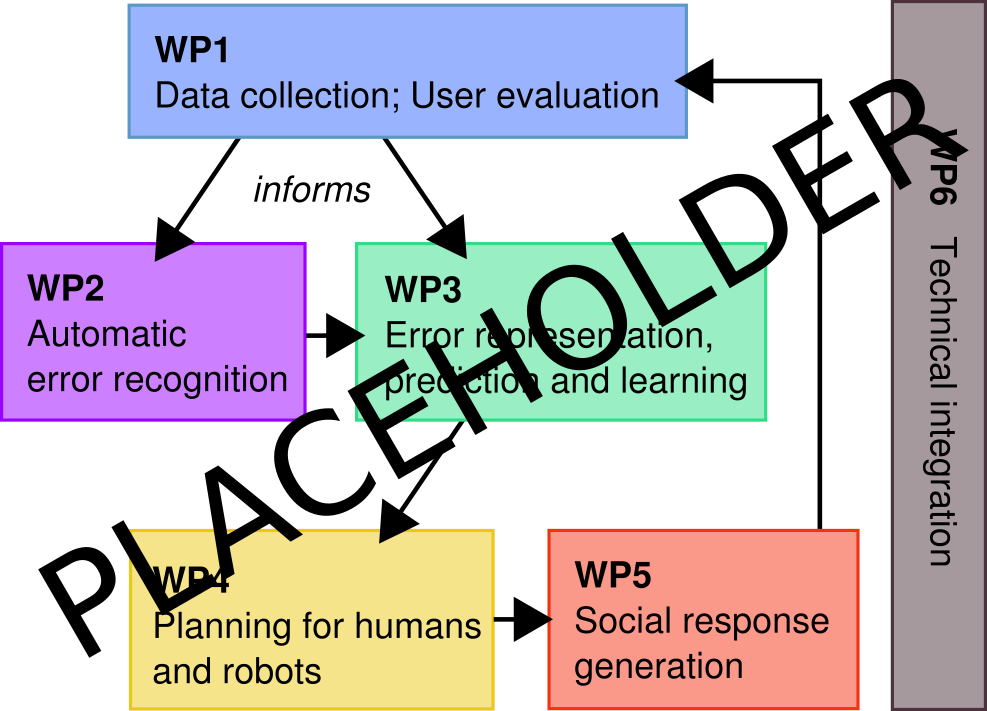
\includegraphics[width=0.8\linewidth]{figs/wp-interrelations}
    \caption{Inter-dependencies between work packages and main tasks}
    \label{}
\end{figure}



\subsection{Management structure, milestones and procedures}\label{management-structure-milestones-and-procedures}

\subsubsection{Milestones}\label{milestones}

\begin{itemize}

\item   week-long tests with local children in local schools
\item   field deployment with one child in one school
\end{itemize}

\begin{table}[!htbp]
\caption{List of milestones}
\centering
\begin{tabular}{@{}lllll@{}}
\toprule
\textbf{Milestone number} & \textbf{Milestone name} & \textbf{Related work package(s)} & \textbf{Estimated date} & \textbf{Means of verification} \\ \midrule
                          &                         &                                  &                         &                                \\
                          &                         &                                  &                         &                                \\
                          &                         &                                  &                         &                                \\
                          &                         &                                  &                         &                                \\ \bottomrule
\end{tabular}
\end{table}


\subsubsection{Risks}\label{risks}

\begin{table}[!htbp]
\caption{Identified risks and proposed mitigations}
\centering
\begin{tabular}{@{}lll@{}}
\toprule
\textbf{Description of risk} & \textbf{Work package(s) involved} & \textbf{Proposed risk mitigation measures} \\ \midrule
risk 1 (low/medium/high)     &                                   &                                            \\
                             &                                   &                                            \\
                             &                                   &                                            \\
                             &                                   &                                            \\ \bottomrule
\end{tabular}
\end{table}





\begin{itemize}
    \item week-long tests with local children in local schools
    \item field deployment with one child in one school
\end{itemize}


Plan to hire one mechatronics engineer and one interaction designer

Role of the mechatronics engineer: develop a novel platform, including -
chassis - power autonomy for one day - on-board compute suitable for
deep learning (NVidia TX2?) - vision (embedded RGB-D camera) - audio
processing

Role of the interaction designer: refine interaction modalities (in
particular, the non-verbal speech), details cross-modal interactions,
define interaction patterns with the child

\hypertarget{measuring-how-effective-the-project-is}{%
\subsubsection{Measuring how effective the project
is}\label{measuring-how-effective-the-project-is}}






%%%%%%%%%%%%%%%%%%%%%%%%%%%%%%%%%%%%%%%%%%%%%%%%%%%%%%%%%%%%%%%%%%%%%%%%%%%%%%%%%%%%%%%%
%%%%%%%%%%%%%%%%%%%%%%%%%%%%%%%%%%%%%%%%%%%%%%%%%%%%%%%%%%%%%%%%%%%%%%%%%%%%%%%%%%%%%%%%
%%%%%%%%%%%%%%%%%%%%%%%%%%%%%%%%%%%%%%%%%%%%%%%%%%%%%%%%%%%%%%%%%%%%%%%%%%%%%%%%%%%%%%%%


\newpage

\hypertarget{the-principal-investigator}{%
\section{The principal Investigator}\label{the-principal-investigator}}

\hypertarget{curriculum-vitae}{%
\subsection{Curriculum vitae}\label{curriculum-vitae}}

(max 2 pages)

\hypertarget{early-achievements-track-record}{%
\subsection{Early achievements
track-record}\label{early-achievements-track-record}}

(max 2 pages)

Dr Séverin Lemaignan is Senior Researcher at the Bristol Robotics
Laboratory, University of the West of England, Bristol. Previously, he
obtained a joint PhD in Cognitive Robotics from the CNRS/LAAS (France)
and the Technical University of Munich (Germany) for which he received
the Best PhD in Robotics 2012 award from French CNRS. He then conducted
his research as Research Fellow at EPFL (Switzerland) and Plymouth
University (UK) where he was Lecturer in Robotics until 2018. Dr Séverin
Lemaignan has been involved in several European projects related to
social and cognitive robotics: CHRIS (Cooperative Human Robot
Interaction Systems), DREAM (Development of Robot-Enhanced therapy for
children with AutisM spectrum disorders), L2TOR (Second language
TutOring using social Robots). He has also been awarded in 2015 a EU
H2020 Marie Sklodowska-Curie Individual Fellowship for his project
DoRoThy (Donating Robots a Theory of Mind). His research interests
primarily concern the socio-cognitive aspects of human-robot
interaction, both from the perspective of the human cognition and the
design of cognitive architectures for the robots. More recently, he has
been focusing his experimental work on child-robot interactions in
educative settings, exploring how robots can support teachers and
therapists to develop effective and engaging novel learning paradigms.

\hypertarget{part-b2-the-scientific-proposal}{%
\section{{[}part B2{]} The scientific
proposal}\label{part-b2-the-scientific-proposal}}

(max 15 pages)

\hypertarget{a.-state-of-the-art-and-objectives}{%
\subsection{a. State of the art and
objectives}\label{a.-state-of-the-art-and-objectives}}

\hypertarget{b.-methodology}{%
\subsection{b. Methodology}\label{b.-methodology}}

\hypertarget{risk-assessment}{%
\subsubsection{Risk assessment}\label{risk-assessment}}

\hypertarget{c.-resources}{%
\subsection{c. Resources}\label{c.-resources}}

\hypertarget{host-institution}{%
\subsubsection{Host institution}\label{host-institution}}

The \emph{Bristol Robotics Laboratory (BRL)} is the largest co-located
and most comprehensive advanced robotics research establishment in the
UK. It is a joint venture between the University of the West of England
and the University of Bristol. BRL's multidisciplinary approach aims to
create autonomous devices capable of working independently, with each
other, or with humans. BRL draws on robotics, electrical \& mechanical
engineering, computer science, psychology, cognitive science and
sociology. BRL has an international reputation as a leading research
centre in advanced robotics research and has over 250 researchers
working on a broad portfolio of topics: HRI, collective robotics, aerial
robotics, neuro-inspired control, haptics, control systems, energy
harvesting and self-sustaining systems, rehabilitation robotics, soft
robotics and biomedical systems. BRL has many collaboration
partnerships, both national and international, and is experienced in
managing large multi-site projects. BRL has support from two embedded
units specialising in business and enterprise, together with an
incubator and successful track record of spin-outs.

\newpage

\hypertarget{references}{%
\section{References}\label{references}}

\end{document}
